\documentclass[11pt,a4paper]{article}

\usepackage[T1]{fontenc}
\usepackage[utf8]{inputenc}
\usepackage[margin=1in]{geometry}
\usepackage{booktabs}
\usepackage{tabularx}
\usepackage{array}
\usepackage{hyperref}
\usepackage{amsmath,amssymb}
\usepackage{graphicx}
\usepackage{listings}
\usepackage{xcolor}
\usepackage{titlesec}
\usepackage{fancyhdr}

\hypersetup{colorlinks=true, linkcolor=blue, filecolor=magenta, urlcolor=cyan, citecolor=blue}

\lstset{
    basicstyle=\ttfamily\footnotesize,
    backgroundcolor=\color{gray!10},
    breaklines=true,
    breakatwhitespace=false,
    frame=single,
    xleftmargin=1.5em,
    numbers=left,
    numberstyle=\tiny\color{gray},
    keywordstyle=\color{blue}\bfseries,
    stringstyle=\color{teal},
    commentstyle=\color{gray}\itshape,
    showstringspaces=false,
    literate={→}{{$\rightarrow$}}1
}

\emergencystretch=3em
\setlength{\headheight}{14pt}
\pagestyle{fancy}
\fancyhf{}
\rhead{\textbf{HELIOS Integration Architecture}}
\lhead{synapticTrack \& RAON Linking}
\rfoot{Page \thepage}

\newcommand{\tc}[1]{\texttt{\hbadness=10000 #1}}
\newcolumntype{L}[1]{>{\raggedright\arraybackslash}p{#1}}
\newcolumntype{Y}{>{\raggedright\arraybackslash}X}

\title{
    \vspace{1cm}
    \Huge \textbf{Integration Architecture} \\
    \Large \textbf{Linking synapticTrack and RAON into HELIOS} \\
    \vspace{0.5cm}
    \normalsize \textit{Surrogate Modeling, Reinforcement Learning, and Digital Twin Deployment Strategy} \\
    \large Heavy Ion Linac Intelligent Orchestration Suite
    \vspace{1cm}
}
\author{\textbf{HELIOS Collaboration} \\ Chong Shik Park (\texttt{cspark7701@gmail.com})}
\date{Revision of 2026-10-13}

\begin{document}
\sloppy
\maketitle

\begin{abstract}
This report explains how to link \textbf{synapticTrack} (a machine-neutral beam-dynamics ML library) and \textbf{raon} (the private RAON facility workspace) into \textbf{HELIOS} for surrogate modeling and reinforcement learning (RL), and recommends where the RAON Digital Twin should live. It is based on a direct re-inspection of the three repositories and on measurements of the trained RAON surrogate. We recommend splitting the twin by layer: a facility-agnostic host in HELIOS, the ML engine in synapticTrack, and facility content in raon, linked in-process through an optional entry-point plugin.
\end{abstract}

\tableofcontents
\newpage

\section{Executive Summary}

\textbf{Recommendation: neither a fully separate Digital Twin nor a merged one.} The twin is split by the kind of code it contains.

\begin{table}[ht]
\centering
\small
\begin{tabularx}{\textwidth}{L{3.6cm}L{3.4cm}Y}
\toprule
\textbf{Twin layer} & \textbf{Location} & \textbf{Rationale} \\
\midrule
Twin framework: host, plugin registry, pre-flight verifier, Gymnasium wrapper, MPC hooks, state synchronization & \textbf{HELIOS} (new \tc{helios.twin}) & Online, safety-coupled, open and publishable; called in-process by the Safety gatekeeper. \\
\addlinespace
ML and inference engine: surrogate contracts, models, normalizers, MAP inference, samplers, TRACK runtime & \textbf{synapticTrack} (pip dependency) & Already machine-neutral and governed by its own \tc{AGENTS.md}. \\
\addlinespace
Twin content: lattices, TRACK decks, datasets, checkpoints, calibrations, plugin factory & \textbf{raon} (separate, private) & Confidential by policy; offline HPC lifecycle; independent release cadence. \\
\bottomrule
\end{tabularx}
\caption{Split of the Digital Twin by layer.}
\end{table}

Linking is \textbf{in-process}: HELIOS discovers an optional RAON plugin through a Python entry point. Nothing crosses the network, and HELIOS has no import-time dependency on raon. Without raon (for example in public CI), HELIOS falls back to its analytic twin.

\begin{table}[ht]
\centering
\small
\begin{tabularx}{\textwidth}{L{7.2cm}Y}
\toprule
\textbf{Quantity (Python 3.11, torch 2.14.1+cpu)} & \textbf{Measured result} \\
\midrule
Load legacy LEBT surrogate (\tc{legacy\_50000/best\_model.pt}) with the raon legacy loader & OK: 13 inputs $\rightarrow$ 12 outputs, 120{,}332 parameters \\
Wrap in \tc{TorchFrozenSurrogate} (physical units) & OK \\
Single-sample inference latency (CPU) & \textbf{0.16 ms} \\
Batched inference (1024 samples, CPU) & \textbf{2.4 \textmu s} per sample \\
Gradient $\partial\|\vec y\|^2/\partial\vec u$ through the frozen surrogate & Finite (needed for Neural MPC) \\
\tc{SurrogateLEBTEnv} step (obs 25, action 13) & \textbf{0.48 ms} per step; $10^5$ steps $\approx$ 48 s \\
Held-out test RMS error ($n=7500$), centroids & 0.002 mm (WS1) to 0.11 mm (WS4) \\
\bottomrule
\end{tabularx}
\caption{Measured feasibility of the existing RAON surrogate.}
\end{table}

\textbf{Warning.} In a stock HELIOS environment the cross-repository import currently \emph{fails}: \tc{pandas} and \tc{periodictable} (synapticTrack runtime dependencies) and \tc{stable\_baselines3} (the \tc{rl} extra) are not installed. The measurements above used an isolated scratch install; see Section~\ref{sec:blueprint}.

\section{Architecture Overview}

\begin{figure}[ht]
\centering
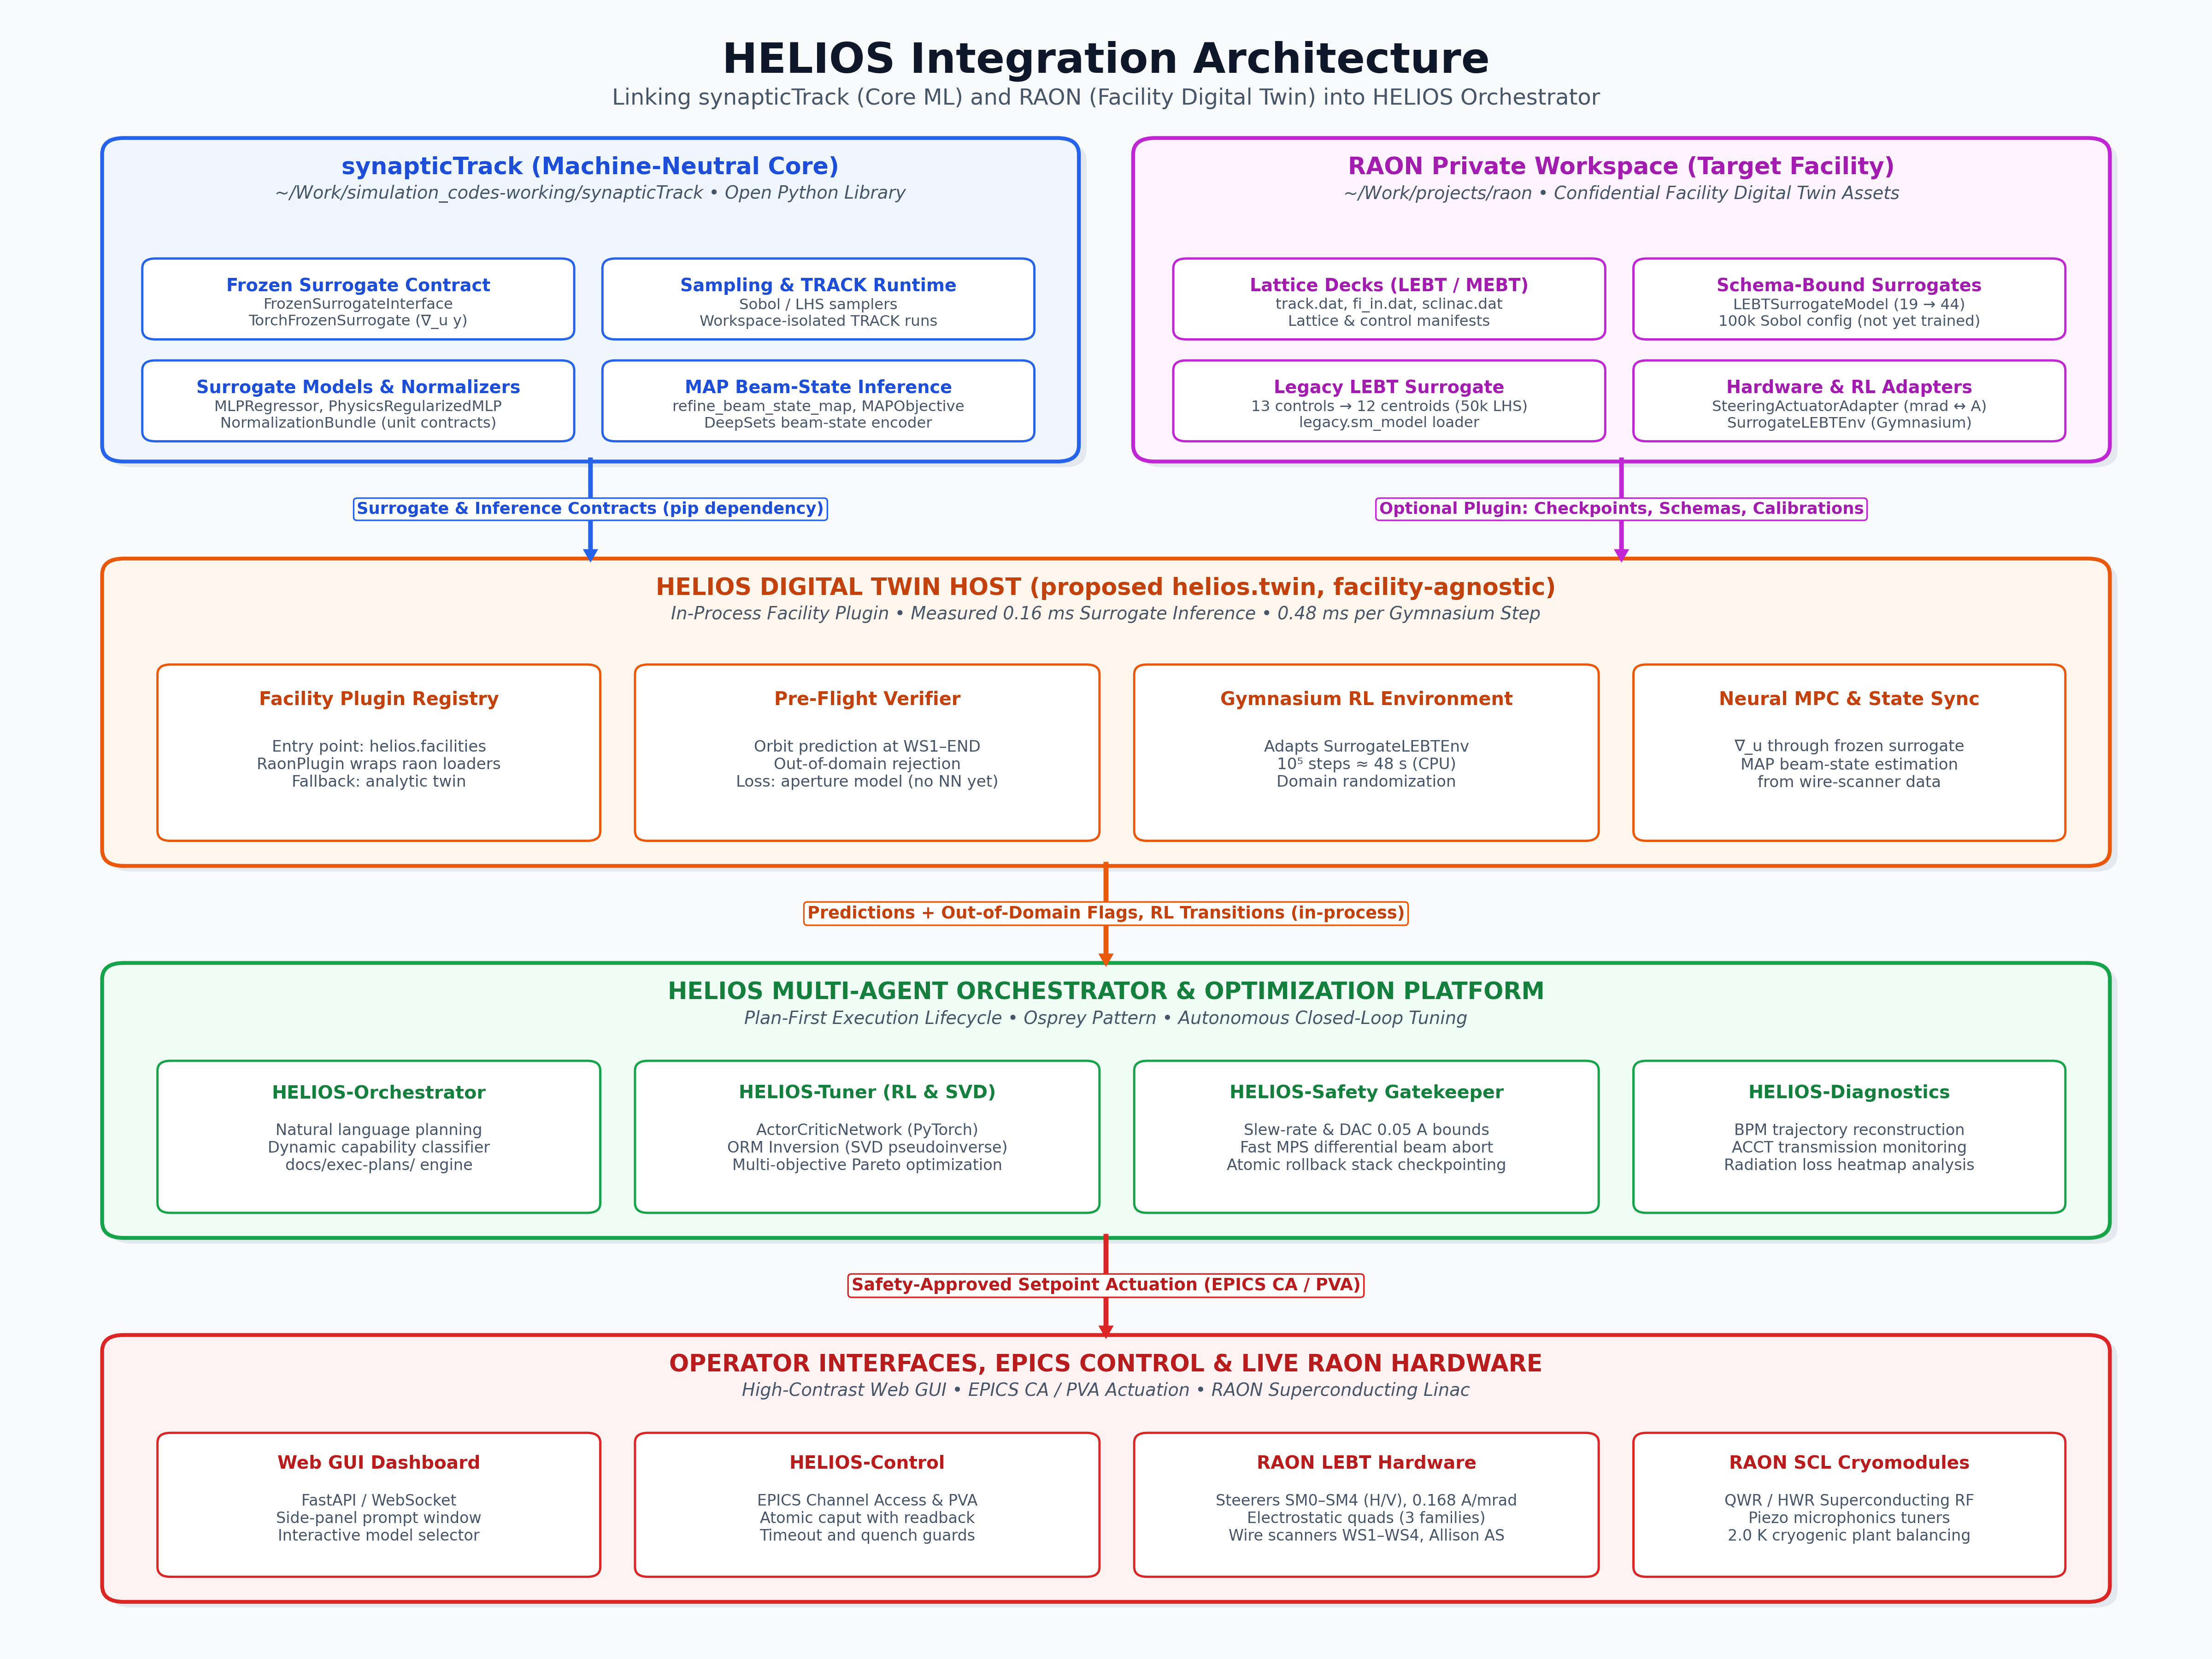
\includegraphics[width=\textwidth]{integration_synaptictrack_raon.png}
\caption{HELIOS integration architecture: synapticTrack (open ML engine) and raon (private facility assets) feed a facility-agnostic twin host in HELIOS, which serves the Tuner and Safety agents before EPICS actuation.}
\label{fig:integration_architecture}
\end{figure}

\textbf{Dependency direction (enforced):}
\begin{itemize}
    \item \tc{helios} $\rightarrow$ \tc{synapticTrack}: optional extra, never mandatory.
    \item \tc{raon} $\rightarrow$ \tc{synapticTrack}: already declared (\tc{synapticTrack>=0.5.0}).
    \item \tc{raon} does \textbf{not} import \tc{helios}; the plugin returns synapticTrack types and plain dataclasses.
    \item \tc{helios} never imports \tc{raon\_adapters} by name; it only iterates the \tc{helios.facilities} entry-point group.
\end{itemize}

\section{What Each Repository Provides}

\subsection{synapticTrack}
Governance: machine-neutral, PyTorch-based, with no machine names, lattice paths, or production defaults in public modules.

\begin{table}[ht]
\centering
\small
\begin{tabularx}{\textwidth}{L{2.6cm}L{5.4cm}Y}
\toprule
\textbf{Capability} & \textbf{Module / API} & \textbf{Use in HELIOS} \\
\midrule
Surrogate contract & \tc{FrozenSurrogateInterface}, \tc{TorchFrozenSurrogate}, \tc{MockLinearSurrogate}, \tc{MockNonlinearSurrogate} & The single surrogate type HELIOS consumes; mocks enable CI without raon. \\
\addlinespace
Models & \tc{MLPRegressor}, \tc{PhysicsRegularizedMLP}, \tc{build\_surrogate\_model} & Instantiated inside the raon plugin. \\
\addlinespace
Normalization & \tc{Normalizer}, \tc{NormalizationBundle} & Differentiable physical-unit boundary. \\
\addlinespace
Beam-state inference & \tc{refine\_beam\_state\_map}, \tc{MAPObjective}, \tc{DeepSetsBeamStateEncoder} & Twin synchronization from scanner data. \\
\addlinespace
Data generation & Sobol/LHS sampling, workspace-isolated TRACK runs & Offline only; stays outside HELIOS. \\
\addlinespace
Artifacts & \tc{artifact\_manifest.json}, strict loaders & Provenance in audit logs. \\
\addlinespace
RL extra & \tc{synapticTrack[rl]}: \tc{gymnasium}, \tc{stable\_baselines3} & RL training backend. \\
\bottomrule
\end{tabularx}
\caption{synapticTrack capabilities relevant to HELIOS.}
\end{table}

\subsection{raon}
Governance: \textbf{confidential}. No public remote, no package publication, and no datasets or trained models in Git.

\begin{table}[ht]
\centering
\small
\begin{tabularx}{\textwidth}{L{2.6cm}Y L{3.6cm}}
\toprule
\textbf{Asset} & \textbf{Details} & \textbf{Status} \\
\midrule
Lattices & \tc{lattice/lebt}, \tc{lattice/mebt}: \tc{track.dat}, \tc{fi\_in.dat}, \tc{sclinac.dat} & Present \\
\addlinespace
LEBT schema & 6 beam-optics inputs, 10 steerer kicks \tc{SM0..4\_H/V} [mrad], 3 EQuad families, 6 diagnostics (\tc{WS1}, \tc{AS}, \tc{WS2}--\tc{WS4}, \tc{END}) & Present \\
\addlinespace
Legacy LEBT surrogate & \tc{legacy\_50000/best\_model.pt}: 13 controls $\rightarrow$ 12 centroids [mm], 50k LHS samples & \textbf{Only trained checkpoint}; loads only via the legacy loader \\
\addlinespace
Schema-bound surrogate & \tc{LEBTSurrogateModel}, config 19 $\rightarrow$ 44 (4$\times$512 SiLU, 100k Sobol) & Code and config only; \textbf{no trained checkpoint} \\
\addlinespace
RL environment & \tc{SurrogateLEBTEnv}, \tc{make\_env}: 12 errors + 13 controls observed, 13 normalized increments, weighted-RMS reward & Present \\
\addlinespace
Hardware adapters & \tc{SteeringCalibrationSet} (0.168 A/mrad, quantized), \tc{SteeringActuatorAdapter} (plans commands, no I/O) & Present \\
\addlinespace
MEBT & Lattice, Sobol production, nominal worker & No trained surrogate \\
\bottomrule
\end{tabularx}
\caption{raon assets verified on disk.}
\end{table}

\subsection{HELIOS}

\begin{table}[ht]
\centering
\small
\begin{tabularx}{\textwidth}{L{4.6cm}Y}
\toprule
\textbf{Existing component} & \textbf{State and integration impact} \\
\midrule
\tc{FastPhysicsSurrogate} & Wraps the analytic MEBT twin; becomes the fallback backend. \\
\tc{NeuralLinacSurrogate} & Untrained network with hard-coded \tc{MEBT:*} keys and a dict API; superseded by \tc{FrozenSurrogateInterface}. \\
\tc{LinacGymEnv} & Analytic MEBT demo environment; remains the open demo. \\
\tc{NeuralMPCController} & Bound to the dict API; needs an adapter for \tc{FrozenSurrogateInterface}. \\
\tc{LinacRLAgent} & In-house actor-critic; can train on the RAON environment via Gymnasium. \\
\tc{create\_raon\_scl1\_lattice} & SCL1 model; a different section from the trained LEBT surrogate. \\
\tc{pyproject.toml} & \tc{ml} extra only requires \tc{torch>=2.0}; needs a \tc{twin} extra. \\
\bottomrule
\end{tabularx}
\caption{HELIOS components affected by the integration.}
\end{table}

\section{Digital Twin: Separate or Included?}

\begin{table}[ht]
\centering
\footnotesize
\begin{tabularx}{\textwidth}{L{3.3cm}YYY}
\toprule
\textbf{Criterion} & \textbf{A. Merge into HELIOS} & \textbf{B. Separate service} & \textbf{C. Layered plugin (recommended)} \\
\midrule
RAON confidentiality & Violated & Satisfied & Satisfied \\
synapticTrack neutrality & Pressure to add RAON defaults & Satisfied & Satisfied \\
Pre-flight latency & $\sim$0.2 ms & Network round trip & $\sim$0.2 ms (measured) \\
Gradients for MPC & Yes & Not across RPC & Yes \\
RL throughput & $\sim$48 s per $10^5$ steps & RPC-bound & $\sim$48 s per $10^5$ steps \\
Offline HPC lifecycle & Bloats control repo & Separate & Stays in raon/synapticTrack \\
Public CI & Needs private assets & Needs mock service & Uses synapticTrack mocks \\
Release cadence & Coupled & Decoupled & Decoupled via plugin protocol \\
Operations overhead & Low & High & Low \\
\bottomrule
\end{tabularx}
\caption{Architectural options.}
\end{table}

\subsection{Decision}
Adopt \textbf{Option C}. Do not create a fourth ``digital-twin'' repository now. The facility-specific part already has a policy-mandated home (raon), the reusable ML part has one (synapticTrack), and the missing thin open \emph{host} layer belongs in HELIOS, where the Safety and Tuner agents call it.

\subsection{When to revisit (triggers for Option B)}
\begin{enumerate}
    \item Several independent consumers need the same live twin state concurrently (GUIs, a virtual accelerator publishing soft-IOC PVs, other teams' tools).
    \item Inference must run on a dedicated remote GPU node.
    \item The twin becomes a slow, high-fidelity model whose latency already dominates RPC overhead.
\end{enumerate}
Even then, the Safety gatekeeper should keep an in-process copy of the fast surrogate for pre-flight checks.

\section{Linking Blueprint}
\label{sec:blueprint}

\subsection{Step 1: Environment and packaging}
Install packages instead of editing \tc{PYTHONPATH}; the latter adds source trees but not their dependencies, which is why the import fails today.
\begin{lstlisting}[language=bash]
conda activate helios
pip install -e ~/Work/simulation_codes-working/synapticTrack[rl]
pip install -e ~/Work/projects/raon     # private; local only, never in CI
\end{lstlisting}
In HELIOS \tc{pyproject.toml}, raon is deliberately not listed:
\begin{lstlisting}
[project.optional-dependencies]
twin = ["synapticTrack[rl]>=0.5.0"]
\end{lstlisting}
\tc{setup.sh} stays opt-in and uses environment variables rather than hard-coded home paths, since HELIOS is meant to be publishable:
\begin{lstlisting}[language=bash]
for src in "${HELIOS_SYNAPTICTRACK_SRC:-}" "${HELIOS_RAON_SRC:-}"; do
    if [[ -n "${src}" && -d "${src}" ]]; then
        export PYTHONPATH="${src}${PYTHONPATH:+:${PYTHONPATH}}"
    fi
done
\end{lstlisting}
synapticTrack requires \tc{torch>=2.13} while the HELIOS \tc{ml} extra allows \tc{torch>=2.0}; the HELIOS environment already has 2.14.1, and the \tc{twin} extra inherits the stricter bound.

\subsection{Step 2: Twin host protocol in HELIOS}
\begin{lstlisting}[language=Python]
# helios/twin/protocol.py (open, no raon imports)
@dataclass(frozen=True)
class TwinDomain:
    names: Sequence[str]; lower: np.ndarray; upper: np.ndarray
    def out_of_domain(self, u, margin=0.0) -> list[str]: ...

@dataclass(frozen=True)
class FacilityTwin:
    facility: str; section: str
    surrogate: FrozenSurrogateInterface
    control_names: Sequence[str]; control_units: Sequence[str]
    diagnostic_names: Sequence[str]
    domain: TwinDomain
    provenance: Mapping[str, str]

class FacilityPlugin(Protocol):
    name: str
    def available_sections(self) -> Sequence[str]: ...
    def load_twin(self, section: str) -> FacilityTwin: ...
    def to_actuator_commands(self, section, controls) -> Mapping[str, dict]: ...
    def make_env(self, section: str, **kwargs): ...
\end{lstlisting}
The registry iterates \tc{entry\_points(group="helios.facilities")}; a broken private plugin only logs a warning and never breaks HELIOS.

\subsection{Step 3: RAON plugin (in raon, imports only synapticTrack)}
\begin{lstlisting}[language=Python]
# raon/pyproject.toml
# [project.entry-points."helios.facilities"]
# raon = "raon_adapters.helios_plugin:RaonTwinPlugin"

class RaonTwinPlugin:
    name = "RAON"
    def load_twin(self, section):
        model, xm, xs, ym, ys, cfg = sm_model.load_surrogate_checkpoint(
            str(self.lebt_ckpt), device="cpu")
        sur = TorchFrozenSurrogate(
            _PhysicalUnits(model.cpu(), xm, xs, ym, ys),
            beam_state_dim=1, machine_dim=13, diagnostic_dim=12,
            input_builder=lambda _b, u: u, device="cpu")
        ...  # names, units, TwinDomain from training bounds, sha256
\end{lstlisting}

\subsection{Step 4: Surrogate-based pre-flight verification}
\begin{enumerate}
    \item HELIOS-Tuner proposes candidate kicks (mrad) and EQuad settings.
    \item \tc{helios.twin} checks the candidate against the training-domain bounds. If it is out of domain, it rejects it or falls back to the analytic twin with operator confirmation.
    \item In domain: the surrogate predicts centroids at WS1 to END (0.16 ms).
    \item The predicted orbit is checked against aperture-derived limits.
    \item The plugin converts mrad to quantized supply currents with provenance (no I/O).
    \item HELIOS-Safety applies hard limits, slew rate, MPS, and a rollback checkpoint, then authorizes the atomic \tc{caput} with readback.
\end{enumerate}
Rules:
\begin{enumerate}
    \item \textbf{The surrogates do not predict beam loss.} Both RAON models predict centroids (and, for the 19$\rightarrow$44 model, RMS sizes and second moments). Loss checks therefore use an aperture model (centroid plus $k\sigma$ against the local aperture); RMS sizes are available only after the 19$\rightarrow$44 model is trained.
    \item Out-of-domain inputs are rejected or escalated, never extrapolated silently.
    \item Units are converted only at the plugin boundary, and clipped current limits flagged by the adapter must be honored by the gatekeeper.
    \item The checkpoint SHA-256, factory id, and schema are recorded in the plan audit trail.
\end{enumerate}

\subsection{Step 5: Reinforcement learning}
\begin{itemize}
    \item \textbf{Reuse} \tc{make\_env} through \tc{FacilityPlugin.make\_env("LEBT")} instead of re-implementing it. It encodes the RAON observation, action, and reward contract; only centroids enter the reward, so beam sizes are never driven to zero.
    \item \textbf{Throughput}: 0.48 ms per step on CPU, so $10^5$ steps take about 48 s. TRACK time per case was not measured here; benchmark both on one host before quoting a speed-up.
    \item \textbf{Backends}: SB3 PPO/SAC (synapticTrack \tc{rl} extra) or HELIOS \tc{LinacRLAgent}, both through Gymnasium.
    \item \textbf{Sim-to-real safeguards}: randomize the six optics inputs and calibration slopes and add diagnostic noise; gate on ensemble or MC-dropout disagreement; clip actions to the quantized supply step and slew limits during training; prefer residual policies on top of SVD/ORM correction; deploy only at Autonomy Level 1--2 with every action through Step 4.
\end{itemize}

\subsection{Step 6: Neural MPC and differentiable optimization}
Refactor \tc{NeuralMPCController} to accept a \tc{FrozenSurrogateInterface} and optimize with autograd:
\begin{equation}
\vec{u}^{*} = \arg\min_{\vec{u}\in\mathcal{D}} \sum_{k=1}^{H}
\left\| W\bigl(\vec{y}_{\theta}(\vec{u}_k)-\vec{y}_{\text{target}}\bigr)\right\|^{2}
+ \lambda_a\|\vec{u}_k-\vec{u}_0\|^{2}
+ \lambda_s\|\vec{u}_k-\vec{u}_{k-1}\|^{2}
\end{equation}
where $\mathcal{D}$ is the surrogate validity domain intersected with hardware limits. Gradients through the frozen RAON surrogate were verified to be finite.

\subsection{Step 7: Twin state synchronization}
\begin{enumerate}
    \item HELIOS-Diagnostics collects wire-scanner (WS1--WS4) and Allison-scanner profiles.
    \item \tc{refine\_beam\_state\_map} (with \tc{MAPObjective} and \tc{BeamStatePrior}) or the amortized \tc{DeepSetsBeamStateEncoder} estimates the six beam-optics parameters by inverting the surrogate.
    \item The estimate becomes the \tc{beam\_state} input of the 19$\rightarrow$44 model and the domain-randomization center for RL.
\end{enumerate}
This step needs the trained 19$\rightarrow$44 model; the legacy 13$\rightarrow$12 model has no beam-state inputs.

\section{Gaps and Risks}

\begin{table}[ht]
\centering
\small
\begin{tabularx}{\textwidth}{rL{4.9cm}Y}
\toprule
\textbf{\#} & \textbf{Gap or risk} & \textbf{Impact and mitigation} \\
\midrule
1 & HELIOS env lacks \tc{pandas}, \tc{periodictable}, \tc{stable\_baselines3} & Import fails. Install \tc{synapticTrack[rl]}; add the \tc{twin} extra. \\
2 & Only the legacy 13$\rightarrow$12 checkpoint exists; \tc{LEBTSurrogateModel.load} rejects it & No beam-state inputs, RMS sizes, or loss proxy. Load via the legacy loader; train the 19$\rightarrow$44 model. \\
3 & Surrogate covers LEBT only; HELIOS's RAON lattice is SCL1; no MEBT surrogate & Coverage ends at the LEBT exit. Train MEBT surrogates. \\
4 & No beam-loss prediction & Use an aperture model plus RMS sizes; later add a transmission head. \\
5 & HELIOS currents versus RAON kicks in mrad & Single conversion point in \tc{SteeringActuatorAdapter}. \\
6 & Extrapolation outside the training domain & Silent, confident errors. Use the OOD guard and ensembles. \\
7 & Hard-coded home paths in open HELIOS files & Use environment variables. \\
8 & Checkpoints are untracked local files & SHA-256 provenance and \tc{artifact\_manifest.json}. \\
\bottomrule
\end{tabularx}
\caption{Gaps and mitigations.}
\end{table}

\section{Phased Roadmap}

\begin{table}[ht]
\centering
\small
\begin{tabularx}{\textwidth}{rYL{1.9cm}Y}
\toprule
\textbf{Phase} & \textbf{Deliverable} & \textbf{Repo} & \textbf{Exit criterion} \\
\midrule
0 & \tc{twin} extra, editable installs, env-var \tc{setup.sh} & helios & Cross-repo imports succeed in the HELIOS env \\
1 & \tc{helios.twin} protocol, registry, OOD guard; CI with \tc{MockNonlinearSurrogate} & helios & Public CI green without raon \\
2 & \tc{RaonTwinPlugin} (legacy LEBT), entry point, integration tests & raon & Predictions match the legacy forward pass to $10^{-6}$ \\
3 & Pre-flight wired into \tc{SafetyGatekeeper}; audit provenance & helios & End-to-end plan on the simulated control interface \\
4 & RL via \tc{make\_env}; Neural MPC refactor & helios & PPO policy lowers weighted orbit RMS on held-out seeds \\
5 & Train 19$\rightarrow$44 model; MAP state sync & raon, synapticTrack & Test metrics published; MAP recovers synthetic Twiss \\
6 & MEBT surrogate; loss or transmission head & raon & Coverage through MEBT \\
7 & Shadow-mode beam test (Autonomy L0 to L1) & all & Predictions within tolerance of measured WS centroids \\
\bottomrule
\end{tabularx}
\caption{Phased roadmap.}
\end{table}

Each phase touching machine actuation follows the HELIOS Plan-First model (\tc{docs/exec-plans/active} to \tc{completed}).

\section{Summary of Recommendations}

\begin{enumerate}
    \item \textbf{Split the Digital Twin by layer}: host in HELIOS (\tc{helios.twin}), ML engine in synapticTrack, facility content in raon (separate and private). No fourth repository and no network service for now.
    \item \textbf{Link in-process through an entry-point plugin}, with dependencies flowing helios $\rightarrow$ synapticTrack $\leftarrow$ raon.
    \item \textbf{Standardize on \tc{FrozenSurrogateInterface}} as the only surrogate type HELIOS consumes.
    \item \textbf{Start with what exists}: the legacy LEBT surrogate and \tc{SurrogateLEBTEnv} already work (0.16 ms inference, 0.48 ms per RL step).
    \item \textbf{Train the 19$\rightarrow$44 model next} to unlock state synchronization, RMS-based aperture checks, and domain randomization.
    \item \textbf{Make safety explicit}: OOD rejection, aperture-based loss checks, one unit-conversion boundary, provenance logging, and Autonomy $\le$ L2 for learned policies.
\end{enumerate}

\section{Corrections to the Previous Revision}

\begin{table}[ht]
\centering
\small
\begin{tabularx}{\textwidth}{L{6.2cm}Y}
\toprule
\textbf{Previous statement} & \textbf{Verified fact} \\
\midrule
\tc{LEBTSurrogateModel.load} loads \tc{legacy\_50000/best\_model.pt} & Fails: the checkpoint needs factory \tc{raon\_legacy\_surrogate\_v1}; use the legacy loader. \\
Surrogate predicts beam loss fraction & Neither RAON model predicts loss or transmission. \\
$10^5$ RL steps in under 30 s; over 1000$\times$ faster than TRACK & Measured 0.48 ms per step (about 48 s); TRACK time not measured. \\
Pre-flight under 2 ms & Measured 0.16 ms per surrogate inference. \\
\tc{setup.sh} with hard-coded home paths & Use \tc{pip install -e} and opt-in environment variables. \\
raon provides 3D field maps and PV manifests & Not found; lattices are TRACK decks and hardware mapping is the steering calibration set. \\
Host at \tc{helios.physics.twin} & Does not exist; proposed as the new \tc{helios.twin} package. \\
\bottomrule
\end{tabularx}
\caption{Corrections relative to the earlier document.}
\end{table}

\end{document}
